\documentclass[norsk, 12pt]{article}
\usepackage{babel}          % Ordelingsregler, osv
\usepackage[utf8]{inputenc}
\usepackage[T1]{fontenc}
\usepackage{booktabs}       % Ordentlige tabeller
\usepackage{url}            % Skrive url-er
\usepackage{textcomp}       % Den greske bokstaven micro i text-mode
\usepackage{units}          % Skrive enheter riktig
\usepackage{float}          % Figurer dukker opp der du ber om
\usepackage{lipsum}         % Blindtekst
\usepackage{amsmath, amsfonts, amssymb, amsthm}
\usepackage{caption,subfigure,listings, booktabs}
\usepackage{tikz,graphicx}
\usepackage{sectsty}
\captionsetup{width=.8\textwidth, textfont={small,it},labelfont={small,sf}}

\usepackage{bbold,gillius}
\allsectionsfont{\sffamily} % Sans serif på alle overskrifter
\renewcommand{\abstractname}{Executive Summary}


% Kodelisting
\usepackage{verbatim}
\lstset{language=matlab,breaklines=true,numbers=left} % For hele programmer.
%\lstinputlisting[language=matlab]{fil.m}

% Layout
\usepackage[a4paper,margin=1.5in]{geometry}
\frenchspacing % Rett mellomrom etter punktum.
\linespread{1.1} % Linjeavstand.
\usepackage[colorlinks=true]{hyperref} % Farge på lenker.

% Egendefinerte kommandoer
\theoremstyle{definition} \newtheorem{defi}{Definisjon}[subsection]
\theoremstyle{definition} \newtheorem{teo}{Teorem}[subsection]
\theoremstyle{definition} \newtheorem*{eks}{Eksempel}
\newcommand{\dt}{\, {\rm d}t\, }
\newcommand{\dx}{\, {\rm d}x\, }
\newcommand{\dv}{\, {\rm d}v\, }
\newcommand{\dr}{\, {\rm d}r\, }
\newcommand{\dd}{\, {\text d} }
%\newcommand{\dp}{\ {\rm d}p\ }
\newcommand{\R}{\mathbb{R}}
\def\mean#1{\langle #1 \rangle}
\renewcommand{\exp}{\mathit{e}}
%\DeclareMathOperator{\dt}{dt}
\newcommand{\mb}[1]{\mathbf{#1}}
\def\para#1{\left( #1 \right)}
\newcommand{\ket}[1]{\left|#1\right\rangle}
\newcommand{\bra}[1]{\left\langle#1\right|}

% JF i margen
\makeatletter
\renewcommand{\subsubsection}{\@startsection{subsubsection}{3}{-2cm}%
{-\baselineskip}{0.5\baselineskip}{\bf\large}}
\makeatother
\newcommand{\jf}[1]{\subsubsection*{JF #1}\vspace*{-2\baselineskip}}

% Skru av seksjonsnummerering
\setcounter{secnumdepth}{-1}

%, trim = 1cm 7cm 1cm 7cm % PDF-filer som bilde

\begin{document}

% Forside
\begin{titlepage}
\begin{center}

\textsf{\Large FYS4150 - Computational Physics\\[0.5cm]
\rule{\linewidth}{0.5mm} \\[0.4cm]
{ \huge \bfseries  PROSJEKT 2}\\[0.10cm]
\rule{\linewidth}{0.5mm} \\[1.5cm]
{\Large Å løse Schrödingers likning for étt og to elektroner}}\\[1.5cm]
\textsc{}\\[1.5cm]

% Av hvem?

\textsf{\begin{minipage}{0.49\textwidth}
    \begin{center} \large
        Jon Vegard Sparre\\ \url{jonvsp@uio.no} \\[0.8cm]
    \end{center}
\end{minipage}
\begin{minipage}{0.49\textwidth}
    \begin{center} \large
        Anne-Marthe Hovda\\ \url{annemmho@uio.no} \\[0.8cm]
    \end{center}
\end{minipage}}


\vfill

% Dato nederst
\textsf{\large{Dato: \today}}

\end{center}
\end{titlepage}

\abstract{I dette prosjektet har vi løst Schrödingerlikninga for harmonisk oscillator med ett og to elektroner. Vi har brukt Jacobis metode og egenverdi-løseren til Armadillo-biblioteket for å løse den numerisk. De numeriske resultatene har blitt sammenliknet med de analytiske resultatene til M. Taut\cite{Taut}. Vi har kun sett på løsningene for relativ avstand med og uten Coulomb-frastøtning. I tillegg har vi også sett på presisjon og stabilitet.}

Lenke til Jon Vegards GitHub-domene: \url{https://github.com/jonvegards/FYS4150}

\section*{Introduksjon}
Problemet som vi kommer til å løse i dette prosjektet er Schrödingerlikninga (SL) for en 3D harmonisk oscillator med ett og to elektroner. Vi har et sfærisk symmetrisk potensiale, som gjør at vi trenger kun å løse den radielle SL, \emph{i.e.} vi reduserer det tredimensjonale problemet til et éndimensjonalt et. Den radielle delen av SL er da, for en harmonisk oscillator
$$ -\frac{\hbar^2}{2m} \para{ \frac{1}{r^2} \frac{\dd}{\dr}r^2 \frac{\dd}{\dr} - \frac{l(l+1)}{r^2}}R(r) + \frac{m\omega^2r^2}{2} R(r) = E R(r).$$
Det er essensielt denne likninga vi skal løse gjennom hele prosjeket i forskjellige former. Metoden vi skal bruke her, ble vi kjent med i prosjekt 1. Vi tar utgangspunkt i trepunktsformelen for en annenderivert, diskretiserer funksjonen i $n$ steg med en steglengde $h$, setter det opp som en tridiagonal matrise og løser matriselikninga med ei egna algoritme.

I løpet av prosjektet vil vi utvikle vår egen numeriske løsning ved hjelp av \emph{Jacobis algoritme}. I tillegg til dette vil vi også bruke Armadillo til å løse problemet. Begge metodene vil så bli sammenliknet med den analytiske løsningen til Taut \cite{Taut}. Vi vil også bruke MATLAB for å lage plott (og litt egenverdikontroll underveis). 

\section*{Teori}
SL er gitt i sfæriske koordinater, s.a. $r\in [0,\infty)$. Denne likninga inneholder noen stygge annenderiverte som vi vil endre på, så vi substituerer $R(r) = (1/r)u(r)$ og får,
$$ -\frac{\hbar^2}{2m}\frac{\dd^2}{\dr^2}u(r) + \para{\frac{\hbar^2}{2m}\frac{l(l+1)}{r^2} + \frac{m\omega^2r^2}{2}} u(r) = E u(r).$$
Randbetingelsene her er greie å finne ut av, siden vi ikke vil at  $R(r)$ skal divergere så må $u(0) = 0$, det er lett å se ut i fra hvoran vi har definert $R(r)$. Potensialet vårt øker med $r^2$, dette tilsier at sannsynligheten vil avta jo lengre unna vi er fra origo og dermed blir $u(\infty) = 0$. 

Prøver vi å putte likninga inn i et program slik den er nå, så vil vi få noen ubehagelige overraskelser hva gjelder avrundingsfeil, overflow og andre ting vi ikke vil ha i en numerisk løsning. Vi innfører derfor dimensjonsløse variable, da blir resultatet automagisk på den lengdeskalaen problemet krever at det er. Først setter vi $ \rho = (1/ \alpha)r$, $\alpha$ er en konstant med dimensjon lengde. Ved å sette inn dette får vi
$$ -\frac{\hbar^2}{2m\alpha^2}\frac{\dd^2}{\dd\rho^2}u(\rho) + \para{\frac{\hbar^2}{2m\alpha^2}\frac{l(l+1)}{r^2} + \frac{m\omega^2\alpha^2\rho^2}{2}} u(\rho) = E u(\rho), $$
vi vil ha den annenderiverte for seg selv, så vi ganger med $2m\alpha^2/\hbar^2$ på begge sider og får
$$ -\frac{\dd^2}{\dd\rho^2}u(\rho) + \para{\frac{l(l+1)}{r^2} + \frac{m^2\omega^2\alpha^4\rho^2}{\hbar^2}} u(\rho) = \frac{2m\alpha^2}{\hbar^2}E u(\rho), $$
en siste endring vi gjør er å sette $m^2\omega^2\alpha^4/\hbar^2=1$ og å introdusere $ \lambda = 2m\alpha^2 E/ \hbar^2$. Vi skal i dette prosjektet kun se på løsninger med $l=0$, alt dette gir oss da likninga vi skal implementere i programmet,
$$ -\frac{\dd^2}{\dd\rho^2}u(\rho) + \rho^2u(\rho) = \lambda u(\rho). $$
Den analytiske løsninga for dette problemet gir oss egenverdiene $\lambda_1 = 3$, $\lambda_2 = 7$ og $\lambda_3 = 11$.

Det er ingen grunn til å vente med å se på likninga for problemet med to elektroner, så vi gyver løs på den med en gang. Vi vil så gå gjennom hvordan vi diskretiserer likninga og får den på matriseform, slik vi gjorde i prosjekt 1. For et system med to elektroner vil SL (uten Coulombinteraksjoner) være
\[ \para{- \frac{ \hbar^2}{2m} \frac{\dd^2}{\dr_1^2} - \frac{ \hbar^2}{2m} \frac{\dd^2}{\dr_2^2} + \frac{1}2 k_1r_1^2 + \frac{1}2 k_2r_2^2} u(r_1,r_2) = E^{(2)}u(r_1,r_2), \]
hvor $r_1$ og $r_2$ hendholdsvis er posisjonene til elektron 1 og elektron 2, energien $E^{(2)}$ er den samla energien til systemet og $k_i = m\omega_i^2$. Vi introduserer så den relative koordinaten $r = r_1 - r_2$ og massesenterkoordinaten $R = (1/2)(r_1 + r_2)$, SL tar da formen
$$ \para{- \frac{ \hbar^2}{m} \frac{\dd^2}{\dr^2} - \frac{ \hbar^2}{4m} \frac{\dd^2}{\dd R^2} + \frac{1}4 m\omega_r^2r^2 + m\omega_R^2R^2} u(r,R) = E^{(2)}u(r,R). $$
Dette er heldigvis en separabel differensiallikning, så vi kan sette $u(r,R) = \psi(r)\phi(R)$  og bruke at energien er gitt som $E^{(2)} = E_r + E_R$. Her er vi bare interessert i å løse for $\psi(r)$. Vi legger også til Coulombinteraksjonen, som avhenger av avstanden mellom elektronene,
$$ V(r) = \frac{\beta e^2}r. $$ 
Vi får da
$$ \para{- \frac{ \hbar^2}{m} \frac{\dd^2}{\dr^2} + \frac{1}4 m\omega_r^2r^2 + \frac{\beta e^2}r} \psi(r) = E_r\psi(r). $$
Vi gjentar substitusjonsprosessen som vi gjorde over, $r = (1/\alpha)$. Vi setter $\alpha  = \hbar / m\beta e^2$, $\omega_r^2 = (1/4)(mk\alpha^4/\hbar^2)$ og definerer $ \lambda = m \alpha^2 E/\hbar$, dette gir oss
$$ - \frac{\dd^2}{\dd \rho^2} \psi(\rho) + \para{\omega_r^2\rho^2 + \frac{1}\rho} \psi(\rho) = \lambda \psi(\rho). $$
Vi ser at eneste forskjellen fra i stad er at vi har fått et ekstra potensialledd, hvilket betyr at vi kan lage én algoritme som løser for begge tilfellene.

\section*{Metode}
Nå som vi har stablet på beina likninga vi skal løse, så kan vi ta en titt på den numeriske delen. Vi skal bruke trepunktsformelen for en annenderivert, som vi her kan skrive som
$$ u'' = \frac{u(\rho + h) - 2u(\rho) + u(\rho - h)}{h^2} + \mathcal{O}(h^2), $$
hvor $h$ er steglengden vår. For å diskretisere likninga så kan vi definere
$$ h = \frac{\rho_{\text{max}} - \rho_{\text{min}}}{n_{\text{steg}}}, $$
dette gir oss $\rho_i = \rho_{\text{min}} + ih$, for $i=0,1,\ldots,n_\text{steg}$. Vi kan så skrive SL på formen
$$ -\frac{u_{i+1} - 2u_i + u_{i-1}}{h^2} + V_i u_i = \lambda u_i, $$
hvor $u_{i+1} = u(\rho_i + h)$ etc. og $V_i = \omega_r^2\rho_i^2 + 1/\rho_i$. Dette skriver vi som en tridiagonal matrise der diagonalelementene defineres til å være $d_i = (2/h^2) + V_i$ og elementene på diagonalene over og under hoveddiagonalen til $e_i = -1/h^2$. På matriseform blir dette
\begin{align*}
	\left(\begin{matrix}
	d_1 & e_1 & 0 & \ldots & \ldots & 0 \\
	e_1 & d_2 & e_2 & 0 & \ldots & 0 \\
	0 & \ddots & \ddots & \ddots & \vdots & e_{n_{\text{steg}} - 1} \\
	\vdots & \ddots & \ddots & \ddots & e_{n_{\text{steg}} - 1} & d_{n_{\text{steg}} - 1} \\
	\end{matrix}\right)\left(
	\begin{matrix}
	u_1 \\ u_2 \\ \vdots \\ \vdots \\ u_{n_{\text{steg}}}
	\end{matrix}\right)
	&= \lambda\left(\begin{matrix}
	u_1 \\ u_2 \\ \vdots \\ \vdots \\ u_{n_{\text{steg}}}
	\end{matrix}\right).
\end{align*}
Dette likner veldig på den matriselikninga vi løste i prosjekt 1, men forskjellen nå er at vi har en egenverdilikning. Dette innebærer at når vi løser systemet så er det egenvektorene (opphøyd i andre, slik vi pleier å gjøre med bølgefunksjoner) vi skal plotte mot avstandsvektorene vi lager. For ett-elektrontilfellet vil vi få et plott som viser hvor det er mest sannsynlig å finne elektronet, mens for to-elektrontilfellet vil vi få et plott som viser den mest sannsynlige avstanden mellom elektronene.

Vi kan nå se på algoritmen vi skal bruke for å løse dette systemet. Den kalles \emph{Jacobis algoritme} og går ut på at man skal rotere matrisa $A$ til den er diagonal. En egenverdilikning med ei diagonalmatrise må nødvendigvis ha egenverdiene må diagonalen, så grunnen til å løse den på denne måten her er ganske åpenbar. Algoritmen er beskrevet i større detalj i kompendiet til Morten Hjort-Jensen \cite[p.~215-220]{MHJ15}, så her vil vi bare gjengi hovedpoenga i den. Vi utfører med rotasjonen med ei antisymmetrisk rotasjonsmatrise $S$,
$$ A' = S^T A S. $$ 
hvor $S$ er
\begin{equation*}
S = \left(\begin{matrix}
1 & 0 & \ldots & \ldots & \ldots & \ldots & \ldots & 0 \\
0 & 1 & 0 & \ldots & \ldots & \ldots & \ldots & \vdots \\
\vdots & 0 & 1 & 0 & \ldots & \ldots & \ldots & 0 \\
\vdots & \ldots & 0 & \cos\theta & 0 & \ldots & 0 & \sin\theta \\
\vdots & \vdots & \ldots & 0 & 1 & \ldots & \ldots & 0 \\
\vdots & \vdots & \ldots & \ldots & \ldots & \ldots & 0 & \vdots \\
\vdots & \vdots & \ldots & 0 & \ldots & 0 & 1 & 0 \\
0 & 0 & \ldots & -\sin\theta & 0 & \ldots & 0 & \cos \theta \\
\end{matrix}\right).
\end{equation*}
Denne matrisa gjør en rotasjon i et $n$-dimensjonalt Euklidsk rom. På komponentform har vi
$$ S_{kk} = S_{ll} = \cos\theta,\quad s_{kl} = -s_{lk} = \sin\theta,\quad s_{ii} = 1,\quad i \neq k, i \neq l. $$
Siden vi vil at alle elementer som ikke er på diagonalen til den roterte $A$, skal bli null, så må vi finne en vinkel $\theta$ som gjør at det blir slik. Vi velger oss derfor det største elementet på ikke-diagonalen i $A$ og setter $\theta$ slik at dette elementet blir null, ved å alltid velge det største elementet, sørger vi for at for hver iterasjon, gjør matrisa litt mer diagonal. Vi kan da finne resten av elementene i den nye matrisa $A'$ ut i fra den $\theta$ vi finner. Ved å se på $(2\times2)$-tilfellet av matrisa $A'$ så får vi bare ett ikke-diagonalt element å sette lik null (husk at matrisa er symmetrisk), og det er
$$ A'_{kl} = A_{kl}(c^2 - s^2) + (A{kk} - A_{ll}) cs = 0, $$
gjør vi litt om på denne likninga, og bruker at $\tan\theta = t = s/c$, så får vi
$$  1 - t^2 - t \frac{A_{ll} - A_{kk}}{A_{kl}} = 0 \Rightarrow t^2 + 2\tau t - 1 = 0.  $$
Vi definerte i overgangen her $A_{ll} - A_{kk}/(2A_{kl}) = \tau$. Denne andregradslikninga må vi løse for å finne vinkelen $\theta$ vi skal rotere matrisa $A$ med og samtidig sette det største elementet i $A'$ til null. Når vi løser denne andregradslikninga så får vi to løsninger. Hvilken skal vi velge? Jo, vi velger den som lager minst bry for oss, og det er den minste vinkelen. Jo mindre vi roterer matrisa for hver gang, jo mindre vil andre elementer i $A$ som i utgangspunktet var null, bli forskjøvet fra null. På denne måten gjør vi det så effektivt som mulig. Dette er i grunn hele essensen i algoritmen: finne største element i $A$, regne ut $\theta$, rotere, gjenta til $A$ er diagonal.

Videre vil vi se litt på hvordan vi kan utføre matrisemultiplikasjonen på en lur måte. Matrisa $S$ vil bare endre på elementer i rader og kolonner $k,l$ og $l,k$ i $A$, dette kan vi bruke når vi skal implementere algoritmen i programmet vårt. Vi vil da skrive ei \verb|for|-løkke som går over alle indeksverdier $i$, og for hvert element som har $ A_{ik}$ og $A_{il}$ med $ i \neq l,k$, så får vi ei endring. Vi gjør altså følgende utregninger for hver gang vi skal gjøre en rotasjon,
\begin{align*}
	A'_{ik} &= cA_{ik} - sA_{il}\\
	A'_{ki} &= A'_{ik}\\
    A'_{il} &= cA_{il} + sA_{ik}\\
    A'_{li} &= A'_{il},
\end{align*}
hvor $i\neq k,l$, $c = \cos\theta$ og $s=\sin\theta$. Vi har her utnytta at den nye matrisa også vil bli symmetrisk. For elementene på diagonalen i $A$ får vi
\begin{align*}
	A'_{kk} &= c^2A_{kk} - 2csA_{kl} + s^2A_{ll}\\
	A'_{ll} &= s^2A_{kk} + 2csA_{kl} + c^2A_{ll}\\
	A'_{kl} &= 0\\
	A'_{lk} &= 0,
\end{align*}
Hvor vi i de to siste linjene hardkoder at elementene skal være null siden det er disse elementene vi tar utgangspunkt i for å finne rotasjonsvinkelen $\theta$. Dette er så å si alt vi trenger for å finne egenverdiene vi er på jakt etter. Nå vil vi se på hvordan vi finner egenvektorene. Disse vil nemlig endre seg for hver rotasjon. Siden vi starter med egenverdilikninga $AR = \vec\lambda R$, hvor $R$ inneholder alle egenvektorene som kolonnevektorer og $\vec \lambda$ er en vektor med de tilhørende egenverdiene, så ser vi at etter endt rotasjonsalgoritme så må vi ha $A_\lambda \mathbb{1}^{n\times n} = \vec\lambda \mathbb{1}^{n\times n}$, hvor matrisa $A_\lambda$ har egenverdiene på diagonalen. Vi kan altså gjøre en motsatt rotasjon på $\mathbb{1}^{n\times n}$ for å finne egenvektorene samtidig som vi roterer $A \to A_\lambda$. Denne rotasjonen skjer akkurat på samme måte som for $A$,
\begin{align*}
	R'_{ik} = cR_{ik} - sR_{il}\\
	R'_{il} = cR_{il} + sR_{ik},
\end{align*}
hvor vi looper over $i \neq k,l$. Nå har vi alt vi trenger for å kunne løse egenverdilikninga vi er gitt!

Før vi ser på resultatene, så skal vi se på hvordan programmet fungerer i praksis. Vi har skrevet programmet slik at vi definerer alle variable og parametre for ett-elektron- og to-elektrontilfellet hver for seg og kaller så på funksjone \verb|JacobiRotation| som igjen kaller på de andre funksjonene for å gjøre utregningene. Ved å bygge opp programmet på denne måten blir det enklere å gjøre enhetstester på det.

Gangen i programmet er som følger: Vi definerer alle vektorer, matriser og variable som er nødvendig for utregningene, \emph{i.e.} $A$, $\vec \rho$ og steglengde $h$. Vi setter $n$ til å være dimensjonene til matrisene, slik at $\vec\rho$ må være $n+2$ lang for å få med endepunktene. Endepunktene vet vi at skal være null, så de er ikke med i matrisa $A$. Når vi kaller på funksjonen \verb|JacobiRotation| så sender vi inn $n$, $A$, $\vec w$ og $R$, henholdvis matrisedimensjon, matrisa selv, vektor til å inneholde indeksverdier og identitetsmatrisa $R$. De tre sistnevnte blir endret på globalt av funksjonen slik at vi får hentet ut verdiene vi skal ha når vi skal printe ut resultatene. Før første rotasjon kaller vi på funksjonen \verb FindingMaximumElementOnNonDiagonal , den finner største elementet i matrisa $A$ ved å loope over den øvre triangulære delen av matrisa (minner om at $A^T = A$). Funksjonen gir oss indeksene $k$ og $l$ som forteller oss hvilket element vi skal sette til null og hvor vi skal plassere $\sin\theta$ og $\cos\theta$ i rotasjonsmatrisa $S$. \verb|JacobiRotation| går så inn i ei \verb while -løkke som kaller tre funksjoner for å gjennomføre en iterasjon. Denne løkka går så lenge det største matriseelementet i $A$ er større enn en toleranse $\epsilon$ vi definerer. Det første \verb while- løkka gjør er å sette $c=s=0$ for å forsikre oss om at det ikke blir noe kluss i rotasjonen, deretter kaller den på funksjonen \verb findSinCos  som finner verdiene til $\sin\theta$ og $\cos\theta$ som skal brukes når vi foretar rotasjonen. I denne funksjonen er det en \verb if -test som sørger for at vi velger den minste rotasjonen som er mulig. Neste linje i løkka vår kaller på \verb rotateAmatrix  som foretar selve rotasjonen slik vi har skildra tidligere. Etter å ha rotert så må vi finne det største elementet i den roterte matrisa og så sjekker testen i \verb while -løkka om matrisa er blitt diagonal nok før den går videre til en ny iterasjon.

Som allerede nevnt så må vi også finne egenvektorene til egenverdiene vi regner ut. Dette har vi løst ved å bruke Armadillos sorteringsfunksjon. Ved å lage en \verb uvec -vektor \verb w  til å ta vare på indeksverdier så kan vi skrive \verb|w=sort_index(A.diag());|. Dette vil gi oss en vektor \verb w  som inneholder som første element indeksen til den kolonna i \verb A  som inneholder den laveste egenverdien, andre element, viser til nest laveste egenverdi og så videre. Disse indeksverdiene bruker vi så på matrisa \verb R  når vi skal ha tak i de tilhørende egenvektorene. Så når vi skriver \verb|R.col(w(0))| så får vi ut en kolonnevektor som er egenvektoren til den laveste egenverdien.

For å se til at programmet vårt fungerer som det skal, så har vi lagt inn enhetstester. Disse testene tester programmet for kjente tilfeller, slik at vi vet hva som bør være resultatet. Vi har funksjoner som tester \verb FindMaximumElementOnNonDiagonal  og \verb JacobiRotation  på to måter. Førstnevnte funksjon får tilsendt ei matrise hvor vi veit hva det største elementet er, og så printer testfunksjonen \verb MaxElementTest  ut hva den finner. Sistnevnte blir først testa av \verb TwoByTwoMatrixTest  med ei $2\times2$-matrise for å sjekke om det holder med én iterasjon for å få ei diagonal matrise, resultatet blir printa ut så man kan se om den fungerer. \verb JacobiRotation  blir også testa på tilfellet harmonisk oscillator med ett elektron, vi kjenner egenverdiene til å være $\lambda_0 = 3$, $\lambda_1 = 7$ og $\lambda_2 = 11$, testfunksjonen \verb EigenvalueTest  printer da ut egenverdiene \verb JacobiRotation  finner.

\section*{Resultater}

Våre resultater kan vises ved hjelp av noen av plottene vi plottet i MATLAB.

Figur \ref{fig:reldisthele} viser sannsynlighetsfordelingen til den relative distansen mellom to elektroner, sannsynligheten $|\Psi|^2$ plottet mot den relative distansen $\rho$. Dette plottet viser oss hvor stor relativ distanse det er størst sannsynlighet for at det er mellom de to elektronene. Vi har her plottet både den numeriske og den analytiske løsningen fra Taut \cite{Taut}, slik at vi kan sjekke de opp mot hverandre. Ut i fra plottet i figur \ref{fig:reldisthele} ser vi at den numeriske løsningen stemmer godt overens med den analytiske. Figur \ref{fig:reldist} viser det samme plottet, men her har vi zoomet inn for sjekke hvor lik den numeriske løsningen er til den analytiske. Her ser vi at den numerisk løsningen ikke er helt lik den analytiske slik som figur 1 kunne få oss til å tro. Dersom man ser på aksene her så ser man at forskjellen mellom de to løsningene er ganske liten og det er rimelig å si at vår numeriske løsning er en god tilnærming til den analytiske. Her har vi valgt å sette maks-verdien til den relative distansen til $\rho_{max} = 12$. Valget av $\rho_{max}$ vil bli diskutert mer i detalj, se tabell \ref{tab:rhomax} for en oversikt over hva som skjer ved forskjellige verdier for $\rho_{max}$.

\begin{figure}[H]
\centering
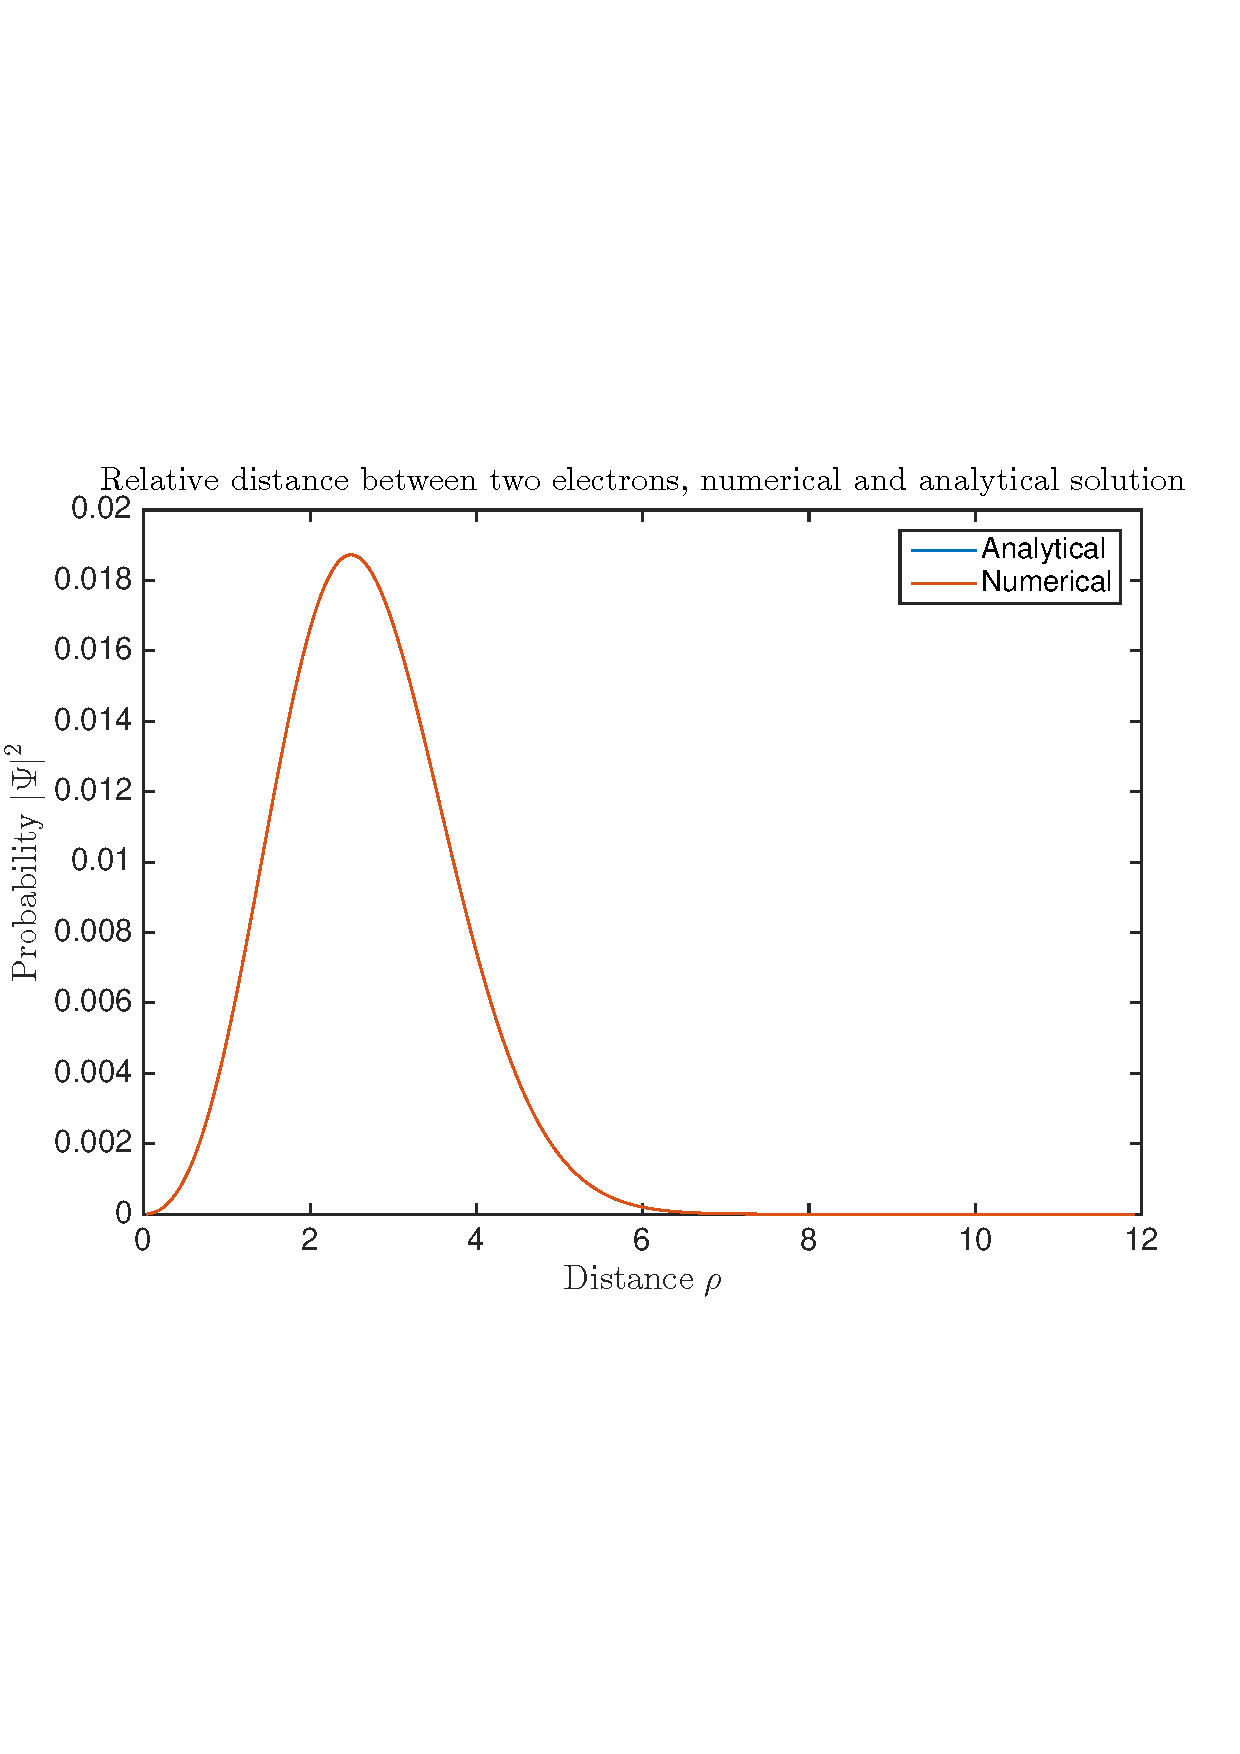
\includegraphics[scale = 0.5, trim = 1cm 7cm 1cm 7cm]{rel_dist_num_anal_hele.pdf}
\caption{Den relative distansen mellom to elektroner, numerisk og analytisk løsning. Vi ser at den numeriske løsningen legger seg fint oppå den analytiske.}
\label{fig:reldisthele}
\end{figure}

\begin{figure}[H]
\centering
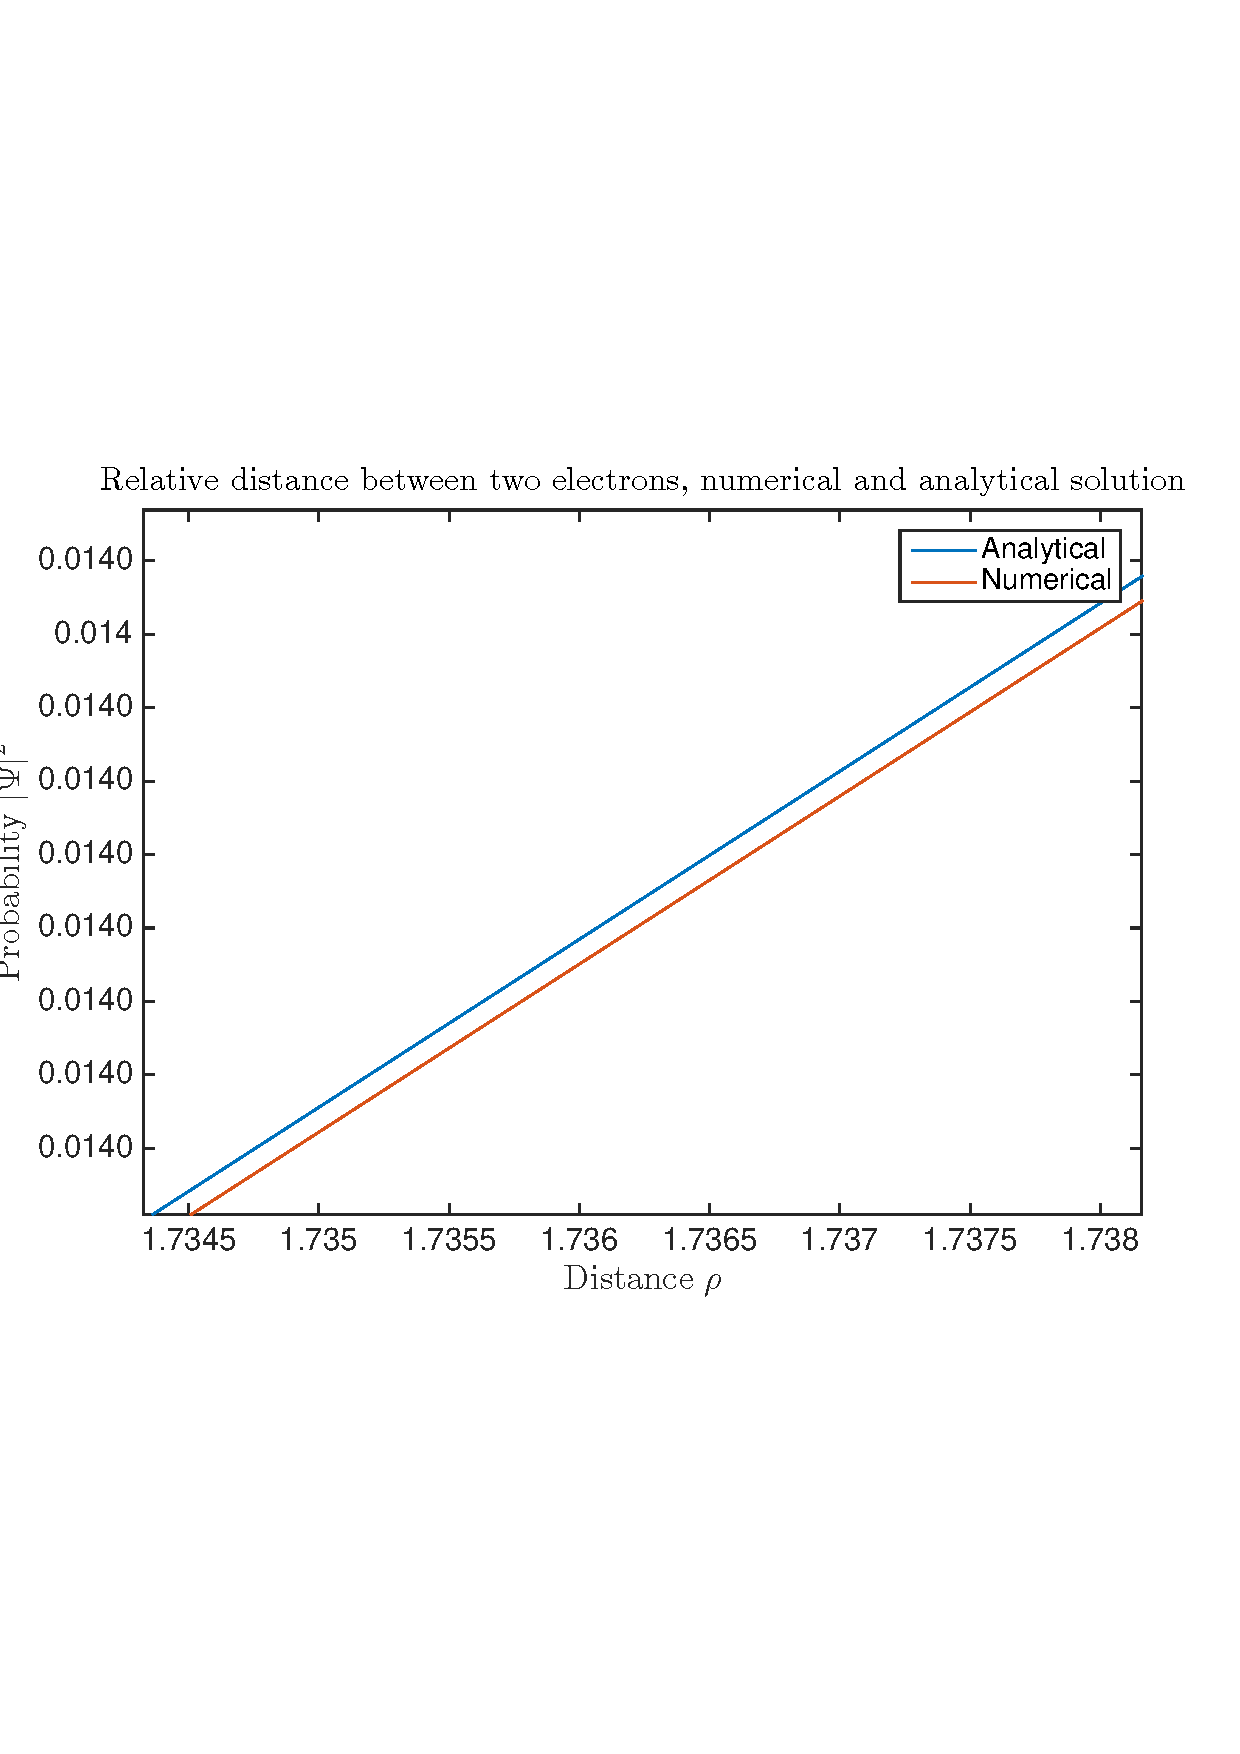
\includegraphics[scale = 0.6, trim = 1cm 7cm 1cm 7cm]{rel_dist_num_anal.pdf}
\caption{Den relative distansen mellom to elektroner, når vi har zoomet inn.}
\label{fig:reldist}
\end{figure}


I figur \ref{fig:omega001} har vi et plott som viser sannsynlighetsfordelinga til den relative distansen mellom to elektroner med en fast verdi for $\omega_r$, hvor $\omega_r$ er en faktor som justerer styrken til oscillator-potensialet. Her har vi valgt en høy maks-verdi for distansen, $\rho_{maks} = 80$, dette er fordi det var kun ved en slik høy verdi at vi fikk et stabilt resultat, henviser igjen til videre diskusjon av valget senere i rapporten og tab. \ref{tab:rhomax}. Videre viser figur \ref{fig:n400} sannsynlighetsfordelinga til den relative distansen for flere forskjellig verdier for $\omega_r$, dette illustrerer hvordan forskjellig styrke på potensialet vil påvirke distansen mellom elektronene. Her ser vi tydelig at ved høyere verdier av $\omega_r$ er det høyere sannsynlighet for at elektronene er nærmere hverandre enn ved en lavere verdi av $\omega_r$, dette gir mening siden $\omega_r$ er her et mål på styrken til potensialet, og ved et sterkere potensiale vil elektronene \emph{føle} en større kraft og bli dytta nærmere hverandre. Styrken på potensialet vil holde elektronene nærmere og vil i større grad motvirke den frastøtende krafta mellom elektronene. Vi ser også at for større verdier av $\omega_r$ så er sannsynlighetsfordelinga spissere, dette tilsier at distansen er skarpere definert ved høyere $\omega_r$, det er et mindre intervall for distansen mellom elektronene.  

\begin{figure}[H]
\centering
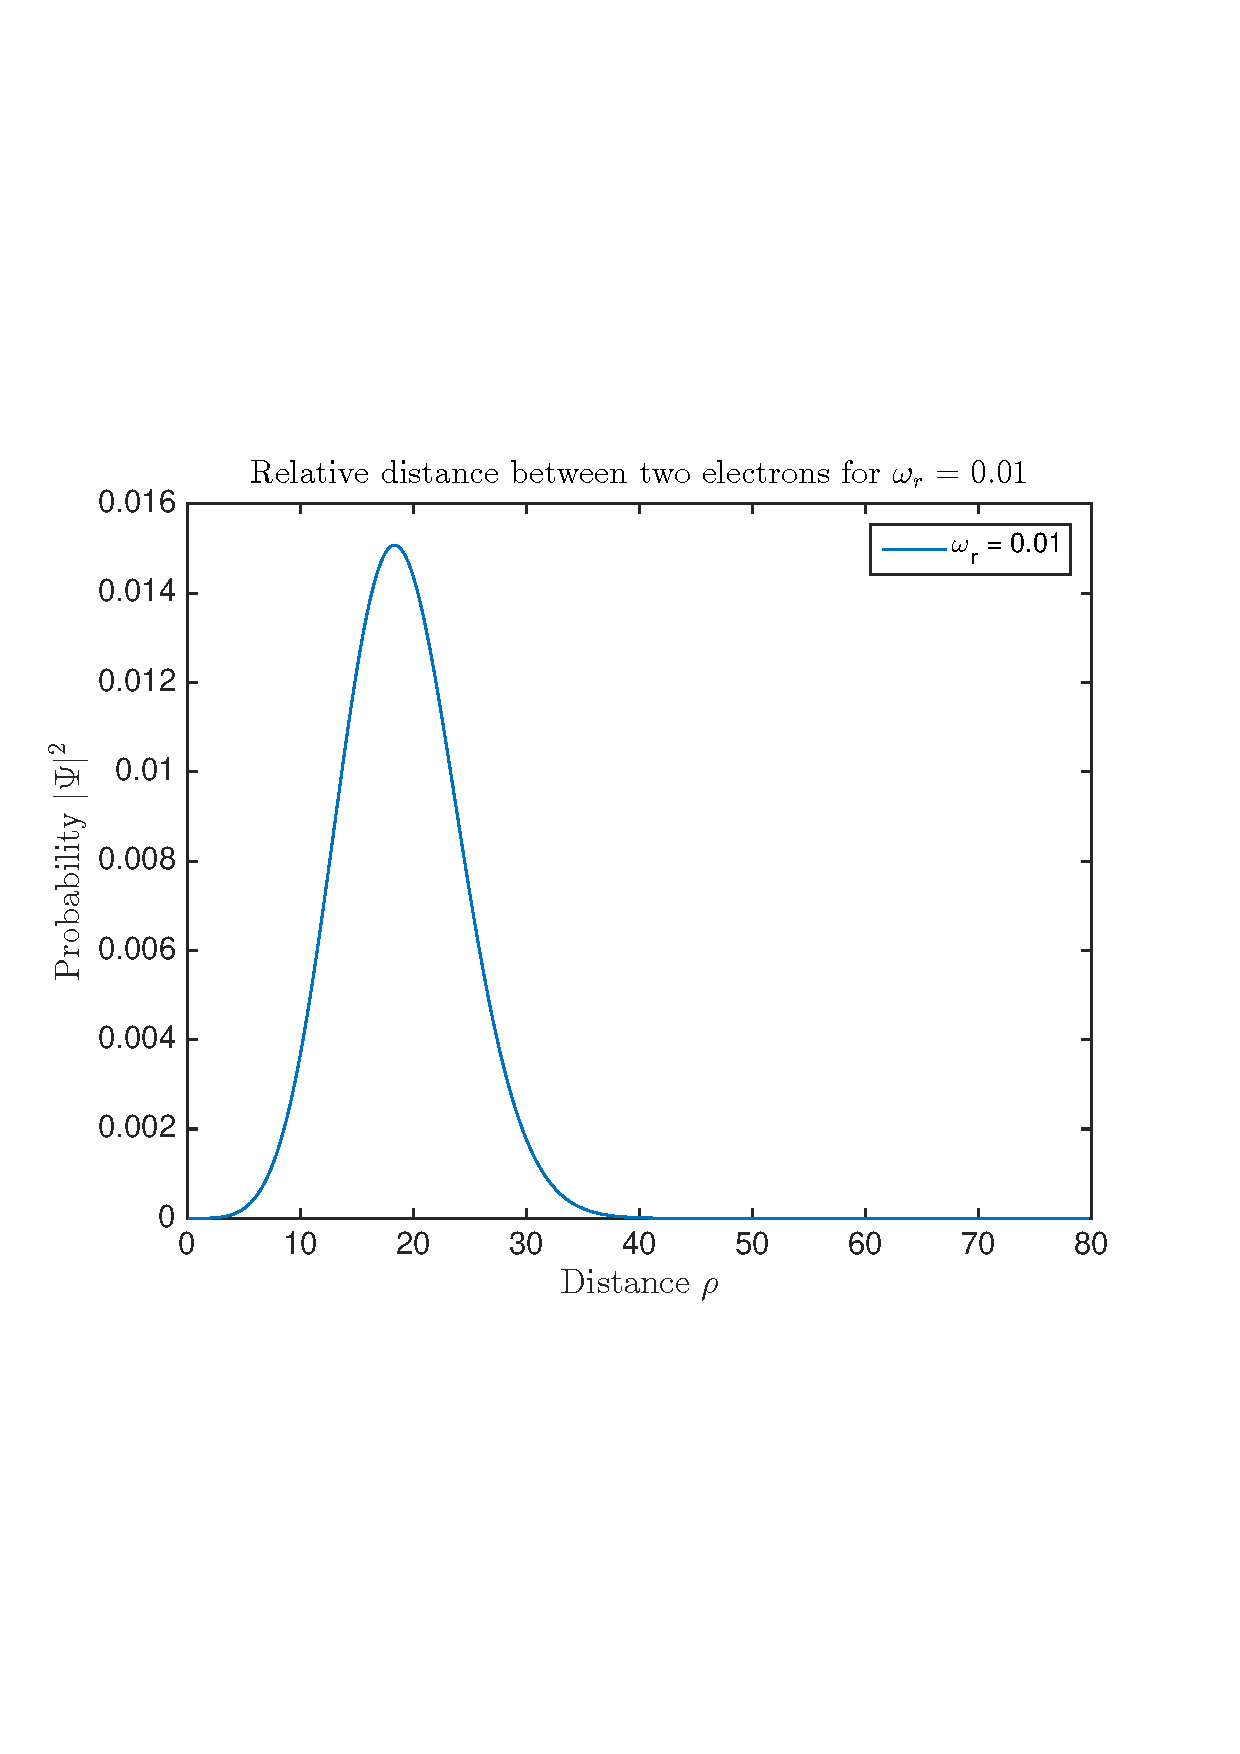
\includegraphics[scale = 0.5, trim = 1cm 7cm 1cm 7cm]{rel_distance_omega001_n400.pdf}
\caption{Den relative distansen mellom to elektroner for $\omega_r = 0.01$ og $n = 400$. Toppunktet til sannsynlighetsfordelinga ligger cirka ved $\rho=20$.}
\label{fig:omega001}
\end{figure}

\begin{figure}[H]
\centering
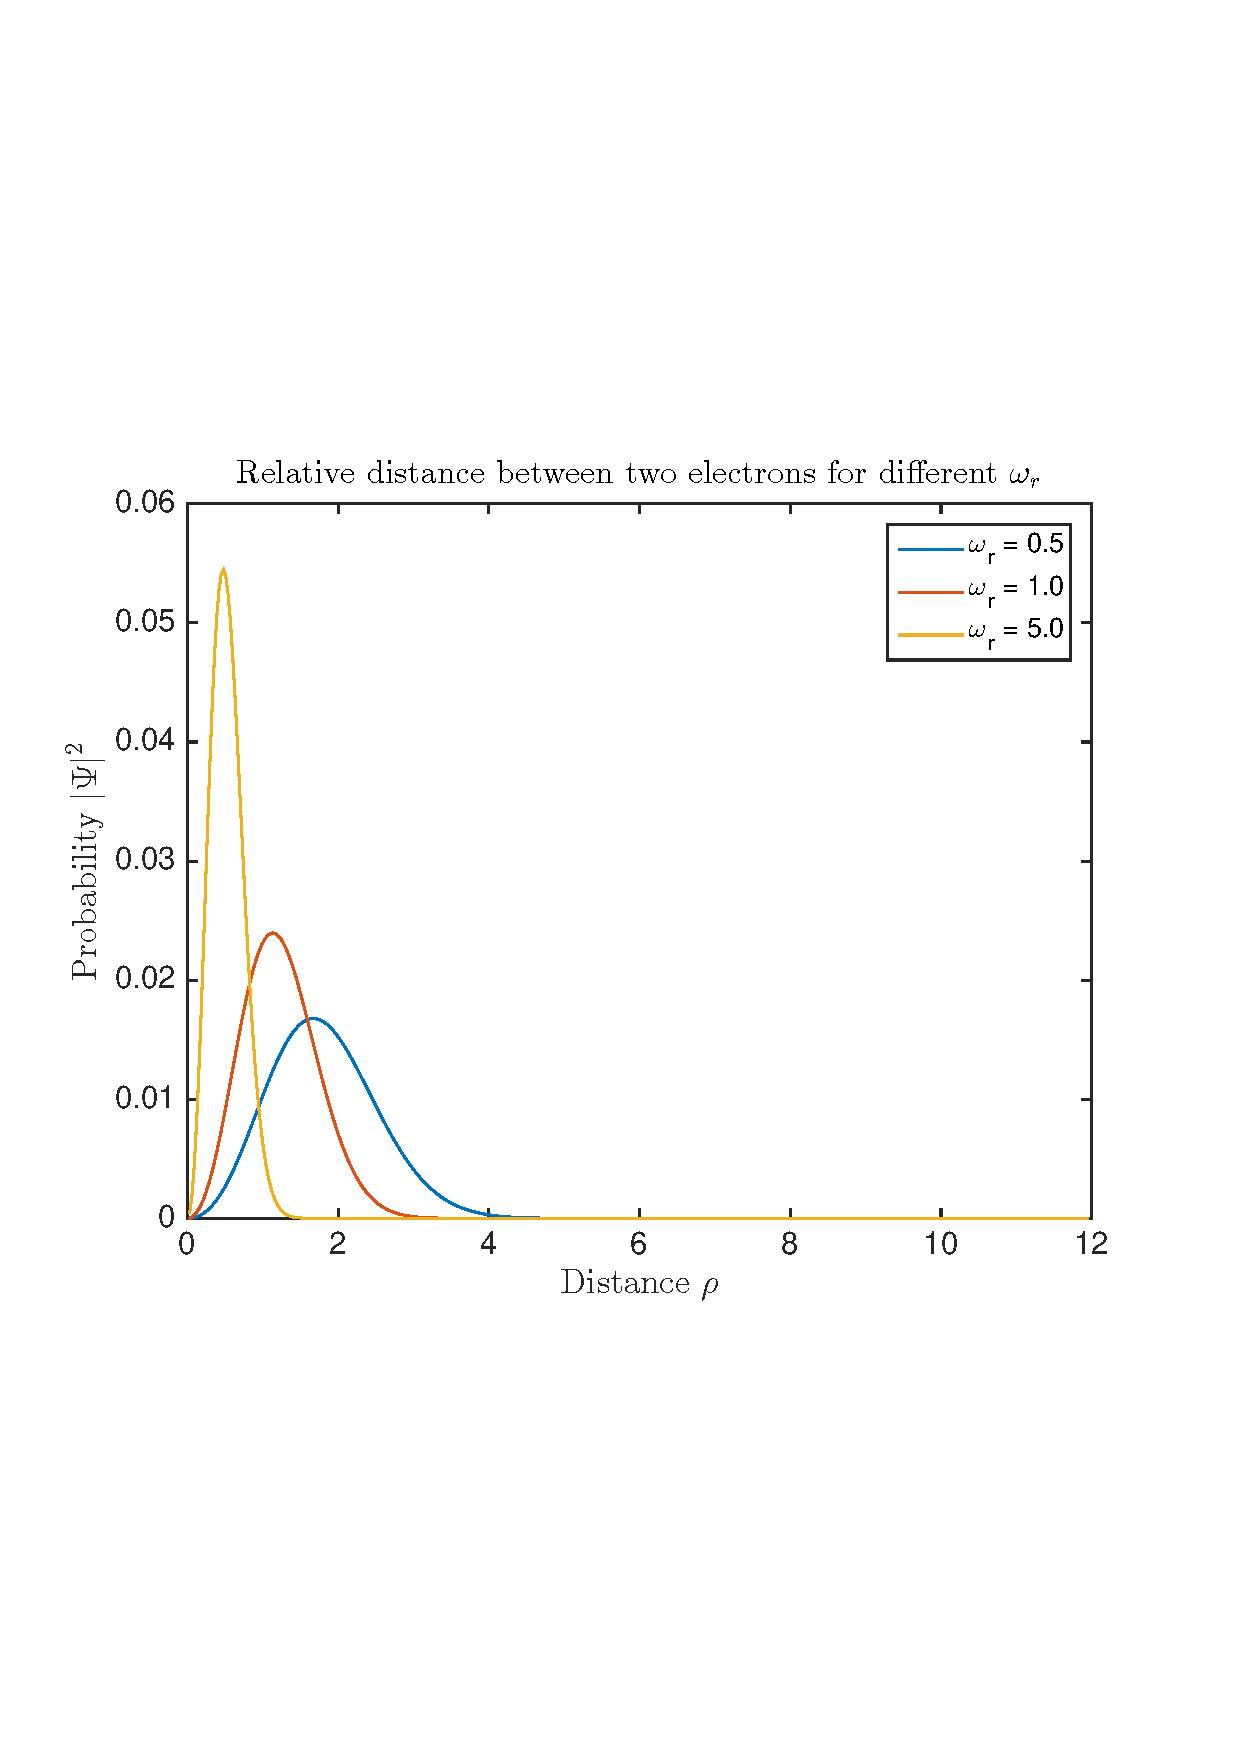
\includegraphics[scale = 0.5, trim = 1cm 7cm 1cm 7cm]{omega_05_1_5.pdf}
\caption{Den relative distansen mellom to elektroner for forskjellige verdier av $\omega_r$ ved $n = 400$. Toppunktene til sannsynlighetsfordelingene ligger nærmere null enn da $\omega_r=0.01$, \emph{i.e.} elektronene er nå nærmere hverandre.}
\label{fig:n400}
\end{figure}


Vi har også lagt ved figur \ref{fig:eig}. Denne figuren viser hvordan valget av egenverdiene, $\lambda$, påvirker sannsynlighetsfordelingen. Egenverdiene tilsvarer energien til egentilstandene, og ved den laveste egenverdien $\lambda_0$ ser vi at det kun er én topp på sannsynlighetsfordelinga, dette gir mening da vi vet at i grunntilstanden er det kun én mulig konfigurasjon av elektronene. I første eksiterte tilstand derimot er det to mulige konfigurasjoner av elektronene og dette gjenspeiles av at sannsynlighetsfordeling har to topper, hvor den ene er litt høyere -- det er den tilstanden som det er høyest sannsynlighet for. Videre følger de neste energitilstandene med økende mulige elektronkonfigurasjoner, dette kommer tydelig frem i fig. \ref{fig:eig} selv om det er noe rotete med alle de forskjellige sannsynlighetsfordelingene. 

\begin{figure}[H]
\centering
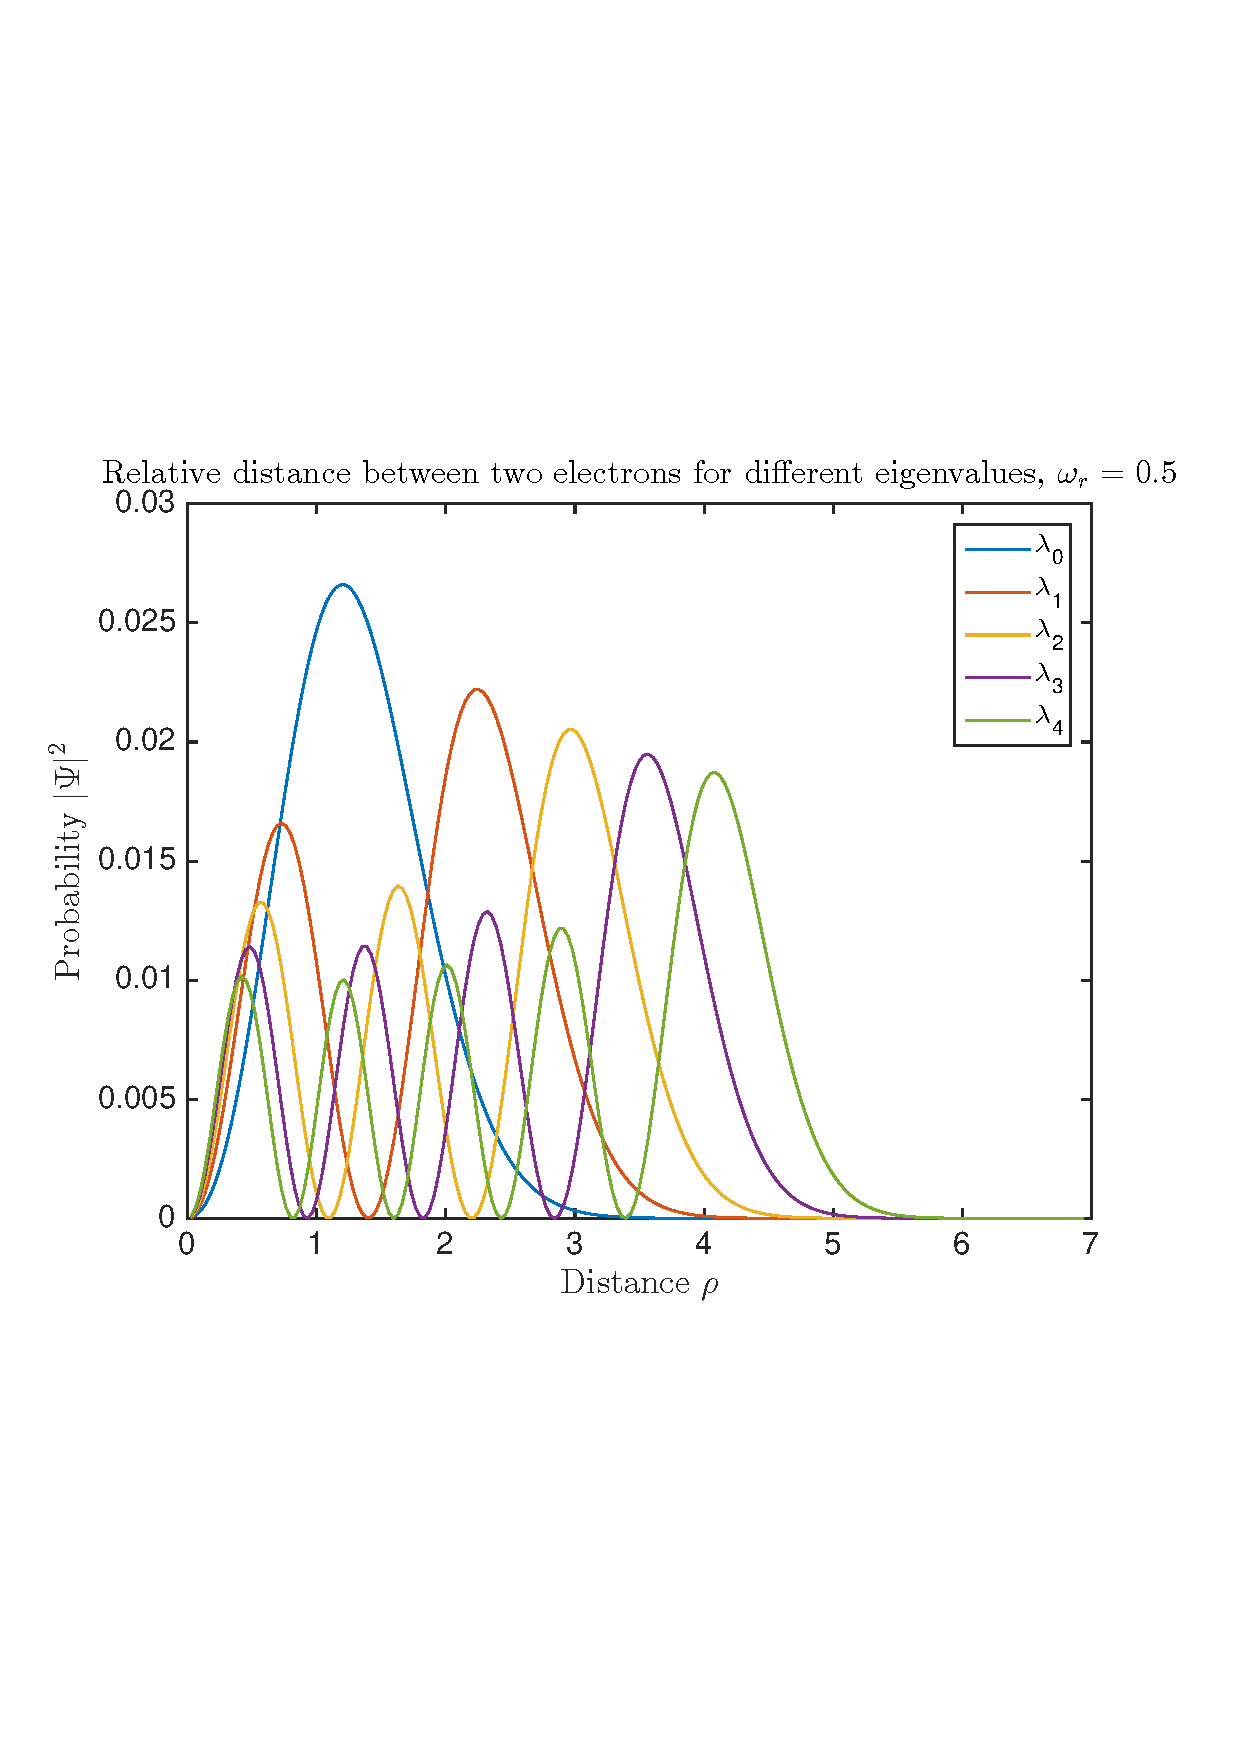
\includegraphics[scale = 0.6, trim = 1cm 7cm 1cm 7cm]{TEC_different_eigenvalues_05.pdf}
\caption{Illustrasjon av egenverdienes påvirkning på sannsynlighetsfordelingen}
\label{fig:eig}
\end{figure}

\subsection*{Numerisk stabilitet og presisjon}
Vi vil her se litt på vårt programs numeriske stabilitet og presisjon. Vi har to hovedparamatre vi kan endre for å forbedre stabiliteten og presisjonen til programmet. Først kan vi se på antall iterasjoner som er nødvendig for at det største elementet i matrisa vi roterer er mindre enn vår $\epsilon = 10^{-8}$. I tab. \ref{tab:ant_iterasjoner} ser vi resultatene for forskjellige $n$. Vi ser at programmet vårt kjører med en god del færre iterasjoner enn teoretisk forventa, noe som kan ha sammenheng med vår valgte $\epsilon$. Velger vi en mindre $\epsilon$ må vi ha flere iterasjoner for å få det største elementet i matrisa til å komme nærmere null.

\begin{table}[H]
  \centering
  \begin{tabular}{ l l l l }
    \toprule
    $n$ & Teoretisk & Faktisk \\
    \midrule
	$10$ & $300$ & $100$ \\
	$100$ & $3000$ & $1.6\cdot10^3$ \\
	$200$ & $300\cdot10^3$ & $65\cdot10^3$ \\
	$400$ & $480\cdot10^3$ & $264\cdot10^3$ \\
	\bottomrule
  \end{tabular}
  \caption{Teoretisk forventa og faktisk antall iterasjoner ved bruk av Jacobis metode. Forventa antall iterasjoner er henta fra \cite[p.217]{MHJ15}. Vi ser at programmet vårt kjører med færre iterasjoner enn forventa, dette kan ha sammenheng med vår valgte verdi for $\epsilon = 10^{-8}$. Hadde vi valgt en mindre $\epsilon$ så måtte programmet iterert flere ganger for å oppnå ønska presisjon.}
  \label{tab:ant_iterasjoner}
\end{table}

Siden vi vet den analytiske løsninga for en tredimensjonal harmonisk oscillator så kan vi teste programmets presisjon. De tre laveste analytiske egenverdiene er $\lambda_0= 3$, $\lambda_1=7$ og $\lambda_2 = 11$. I tab. \ref{tab:presisjon} er forskjellen mellom analytisk og numerisk verdi for forskjellige $n$ lista opp. Som forventa så blir presisjonen bedre ettersom vi øker $n$. Valget av $\rho_\text{max}$ har også innvirkning på presisjonen, i tab. \ref{tab:rhomax} ser vi på harmonisk oscillator med to elektroner og $\omega_r = 0.01$ og hvordan egenverdiene utvikler seg ettersom $\rho_\text{max}$ øker. Potensialet i dette tilfellet er ganske svakt (sammenliknet med de andre tilfellene), så det er naturlig å tenke seg at elektronene vil være lenger fra hverandre. Det betyr at vi må ha en større $\rho_\text{max}$ når potensialet er svakt.

\begin{table}[H]
  \centering
  \begin{tabular}{ l l l l }
    \toprule
    $n$ & $\Delta\lambda_0$ & $\Delta\lambda_1$ & $\Delta\lambda_2$ \\
    \midrule
	$10$ & $0.14704$ & $0.79008$ & $1.98913$ \\
	$100$ & $0.0092$ & $0.00963$ & $0.0235$ \\
	$200$ & $0.00049$ & $0.00245$ & $0.006$ \\
	$400$ & $0.00012$ & $0.00062$ & $0.0015$ \\
	\bottomrule
  \end{tabular}
  \caption{Differanse mellom analytisk og numerisk verdi for egenverdiene i tilfellet med ett elektron i en harmonisk oscillator. Vi ser at presisjonen blir bedre jo større $n$ er. En annen faktor som har innvirkning på presisjonen er valget av $\rho_\text{max}$, se tab. \ref{tab:rhomax}.}
  \label{tab:presisjon}
\end{table}

\begin{table}[H]
  \centering
  \begin{tabular}{ l l }
    \toprule
    $\rho_\text{max}$ & $\lambda_0$  \\
    \midrule
	$10$ & $0.312686$ \\
	$20$ & $0.138030$ \\
	$30$ & $0.108734$ \\
	$50$ & $0.105775$ \\
	$60$ & $0.105774$ \\
	$80$ & $0.105774$ \\
	\bottomrule
  \end{tabular}
  \caption{Programmets stabilitet for egenverdiene i tilfellet med to elektroner i en harmonisk oscillator med $\omega_r = 0.01$. Vi ser at presisjonen er avhengig av verdien vi velger for $\rho_\text{max}$. Velger vi en $\rho_\text{max}$ som er for liten så blir bølgefunksjonen ``presset'' sammen og resultatet vi får ut blir feil. Vi har her kjørt med $n=400$ for alle verdier av $\rho_\text{max}$.}
  \label{tab:rhomax}
\end{table}

Resultatene fra Jacobis metode kan vi sammenlikne med Tauts \cite{Taut} verdier for grunntilstanden med to elektroner og $\omega_r = 0.25$. Taut har i artikkelen sin listet opp egenverdiene $\epsilon'$, i starten av artikkelen definerer han $\epsilon' = (1/2)\epsilon$, hvilket betyr at vi må gange tabellverdiene hans med to for å få verdier som stemmer overens med våre resultater. Den analytiske egenverdien blir da $\lambda_\text{Analytisk} = 1.25$ I tab. \ref{tab:taut} har vi lista opp relativ feil mellom numerisk verdi og analytisk verdi for forskjellige $n$.

\begin{table}[H]
  \centering
  \begin{tabular}{ l l }
    \toprule
    $n$ & Relativ feil \\
    \midrule
    $10$ &  $0.016$ \\
    $20$ &  $0.00468$ \\
	$50$ &  $0.00082$ \\
	$100$ & $0.00022$ \\
	$200$ & $0.00006$ \\
	$250$ & $0.00003$ \\
	\bottomrule
  \end{tabular}
  \caption{Differanse mellom numerisk og analytisk verdi av egenverdiene til grunntilstanden i en harmonisk oscillator med to elektroner. Presisjonen er ganske god hele veien, for $n=10$ er feilen på 1.6\%, og for større $n$ blir den bare mindre og mindre.}
  \label{tab:taut}
\end{table}

Den numeriske presisjonen avhenger også av vårt valg av $\epsilon$, toleransen for hvor lenge \verb while -løkka i funksjonen \verb JacobiRotation  skal iterere. I tab. \ref{tab:jmarm} har vi lista opp differansen mellom Armadillos løsning og den fra Jacobis metode for $n=100$ og $\rho_\text{max}=12$. I den tabellen ser vi at det er en viss forskjell mellom de to numeriske metodene, men at når $\epsilon$ blir liten nok så vil forskjellen være så liten at datamaskinen ikke ser forskjell på de.

\begin{table}[H]
  \centering
  \begin{tabular}{ l l }
    \toprule
    $\epsilon$ & $|\Delta\lambda_0|$ \\
    \midrule
    $10^{-1}$ & $8.8\cdot10^{-4}$ \\
    $10^{-2}$ & $4.47\cdot10^{-6}$ \\
	$10^{-3}$ & $1.63\cdot10^{-7}$ \\
	$10^{-4}$ & $4.63\cdot10^{-10}$ \\
	$10^{-5}$ & $1.30\cdot10^{-11}$ \\
	$10^{-6}$ & $2.57\cdot10^{-13}$ \\
	$10^{-7}$ & $2.04\cdot10^{-13}$ \\
	$10^{-8}$ & $2.04\cdot10^{-13}$ \\
	\bottomrule
  \end{tabular}
  \caption{Differanse mellom Armadillos og Jacobis metodes løsning av laveste egenverdi. For $\epsilon < 10^{-7}$ klarer ikke datamaskinen lenger å gi en nøyaktig differanse mellom resultatene siden de er så like. Til tross for at Jacobis metode er en treg metode, så blir den ganske nøyaktig.}
  \label{tab:jmarm}
\end{table}

\subsection*{Konklusjon}
Vi har nå løst Schrödingerlikninga for en 3D harmonisk oscillator med både ett og to elektroner. Ved implementering av algoritmen har vi gjort noen observasjoner som er viktige for presisjonen av løsningen vår. Vi har sett at parameterne som har innvirkning på presisjon og stabilitet er $n$, $\rho_\text{max}$ og $\epsilon$. Ved å se på hvilke verdier vi må ha for $\rho_\text{max}$ så kan vi justere $n$ deretter. Vi så at algoritmen er ganske presis, men ikke så veldig rask, så vi vil nødig ha en for stor $n$.


Naturligvis er dimensjonen, $n$, til matrisen en viktig faktor, her er det viktig at vi velger en dimensjon som er stor nok til at det opprettholder en viss presisjon, men ikke så stor at programmet tar unødig lang tid å kjøre. 
For at presisjonen til løsningen vår skal være god nok er det også viktig at man velger en maksimumsverdi for distansen mellom elektronene ($\rho_{max}$) som er stor nok, da det følger at for svakere potensiale må man ha en høyere $\rho_{max}$, siden elektronene da vil være lengre fra hverandre. Også valget av $\epsilon$ har en betydning for presisjonen, da dette er toleransen i \verb while - løkken vår.
For at vi skal ha et program som fungerer slik vi ønsker, er det følgelig viktig å teste programmet og endre på variabler som har betydning på presisjonen. Å utføre enhetstester er da en viktig faktor for å sikre seg et program som gir en god tilnærming. 
Vi konkluderer med at stryken på potensiale i en harmonisk oscillator har mye å si for hvor elektronene er, og at Jacobis metode er en nøyaktig, men treg metode.

\begin{thebibliography}{9}
    \bibitem{MHJ15}
    Morten Hjorth-Jensen, \emph{Computational Physics, Lecture Notes Fall 2015}
    
    \bibitem{Taut}
    M. Taut, Physical Review A, 3561 - 3566 (1993)

\end{thebibliography}


\end{document}